% Options for packages loaded elsewhere
\PassOptionsToPackage{unicode}{hyperref}
\PassOptionsToPackage{hyphens}{url}
%
\documentclass[
]{book}
\usepackage{amsmath,amssymb}
\usepackage{lmodern}
\usepackage{ifxetex,ifluatex}
\ifnum 0\ifxetex 1\fi\ifluatex 1\fi=0 % if pdftex
  \usepackage[T1]{fontenc}
  \usepackage[utf8]{inputenc}
  \usepackage{textcomp} % provide euro and other symbols
\else % if luatex or xetex
  \usepackage{unicode-math}
  \defaultfontfeatures{Scale=MatchLowercase}
  \defaultfontfeatures[\rmfamily]{Ligatures=TeX,Scale=1}
\fi
% Use upquote if available, for straight quotes in verbatim environments
\IfFileExists{upquote.sty}{\usepackage{upquote}}{}
\IfFileExists{microtype.sty}{% use microtype if available
  \usepackage[]{microtype}
  \UseMicrotypeSet[protrusion]{basicmath} % disable protrusion for tt fonts
}{}
\makeatletter
\@ifundefined{KOMAClassName}{% if non-KOMA class
  \IfFileExists{parskip.sty}{%
    \usepackage{parskip}
  }{% else
    \setlength{\parindent}{0pt}
    \setlength{\parskip}{6pt plus 2pt minus 1pt}}
}{% if KOMA class
  \KOMAoptions{parskip=half}}
\makeatother
\usepackage{xcolor}
\IfFileExists{xurl.sty}{\usepackage{xurl}}{} % add URL line breaks if available
\IfFileExists{bookmark.sty}{\usepackage{bookmark}}{\usepackage{hyperref}}
\hypersetup{
  pdftitle={Ciencia de Datos y Machine Learning},
  hidelinks,
  pdfcreator={LaTeX via pandoc}}
\urlstyle{same} % disable monospaced font for URLs
\usepackage{longtable,booktabs,array}
\usepackage{calc} % for calculating minipage widths
% Correct order of tables after \paragraph or \subparagraph
\usepackage{etoolbox}
\makeatletter
\patchcmd\longtable{\par}{\if@noskipsec\mbox{}\fi\par}{}{}
\makeatother
% Allow footnotes in longtable head/foot
\IfFileExists{footnotehyper.sty}{\usepackage{footnotehyper}}{\usepackage{footnote}}
\makesavenoteenv{longtable}
\usepackage{graphicx}
\makeatletter
\def\maxwidth{\ifdim\Gin@nat@width>\linewidth\linewidth\else\Gin@nat@width\fi}
\def\maxheight{\ifdim\Gin@nat@height>\textheight\textheight\else\Gin@nat@height\fi}
\makeatother
% Scale images if necessary, so that they will not overflow the page
% margins by default, and it is still possible to overwrite the defaults
% using explicit options in \includegraphics[width, height, ...]{}
\setkeys{Gin}{width=\maxwidth,height=\maxheight,keepaspectratio}
% Set default figure placement to htbp
\makeatletter
\def\fps@figure{htbp}
\makeatother
\setlength{\emergencystretch}{3em} % prevent overfull lines
\providecommand{\tightlist}{%
  \setlength{\itemsep}{0pt}\setlength{\parskip}{0pt}}
\setcounter{secnumdepth}{5}
\usepackage{booktabs}
\ifluatex
  \usepackage{selnolig}  % disable illegal ligatures
\fi
\usepackage[]{natbib}
\bibliographystyle{apalike}

\title{Ciencia de Datos y Machine Learning}
\author{}
\date{\vspace{-2.5em}}

\begin{document}
\maketitle

{
\setcounter{tocdepth}{1}
\tableofcontents
}
\hypertarget{bienvenida}{%
\chapter*{BIENVENIDA}\label{bienvenida}}
\addcontentsline{toc}{chapter}{BIENVENIDA}

\hypertarget{objetivo}{%
\section*{Objetivo}\label{objetivo}}
\addcontentsline{toc}{section}{Objetivo}

Capacitar y brindar acompañamiento al equipo de analítica de ASERTA en temas relacionados con Ciencia de Datos para la correcta implementación de proyectos y toma de decisiones basadas en la evidencia de datos internos y externos a la empresa para lograr un beneficio operativo y económico.

\hypertarget{alcances-del-curso}{%
\section*{Alcances del curso}\label{alcances-del-curso}}
\addcontentsline{toc}{section}{Alcances del curso}

El participante conocerá los conceptos teóricos alrededor de esta ciencia y sabrá implementar correctamente un análisis exploratorio estadístico y gráfico que le permita conocer a mayor profundidad los datos a usar. Conocerá y sabrá implementar los modelos predictivos de Machine Learning más usados y de mayor impacto en la industria de seguros y fianzas. Finalmente, sabrá tomar decisiones sobre el correcto uso e implementación de los modelos para aumentar el beneficio comercial dentro de la institución.

\hypertarget{instructores}{%
\section*{Instructores}\label{instructores}}
\addcontentsline{toc}{section}{Instructores}

\textbf{ACT. ARTURO BRINGAS}

\textbf{LinkedIn:} \href{https://www.linkedin.com/in/arturo-bringas/}{arturo-bringas}
\textbf{Email:} \href{mailto:act.arturo.b@ciencias.unam.mx}{\nolinkurl{act.arturo.b@ciencias.unam.mx}}

Actuario egresado de la Facultad de Ciencias y Maestría en Ciencia de Datos por el ITAM.
Se especializa en modelos predictivos y de clasificación de \emph{machine learning} aplicado a seguros, marketing, deportes y movilidad internacional. Es jefe de departamento en Investigación Aplicada y Opinión de la UNAM, donde realiza estudios estadísticos de impacto social. Ha sido consultor \emph{Sinior Data Scientist} para empresas y organizaciones como GNP, El Universal, UNAM, Sinnia, Geekend, la Organización de las Naciones Unidas Contra la Droga y el Delito (UNODC), entre otros. Actualmente es profesor de \emph{Ciencia de datos y Machine Learning} en AMAT y se desempeña como consultor independiente en diferentes proyectos contribuyendo a empresas en temas de análisis estadístico y ciencia de datos con machine learning.

\begin{center}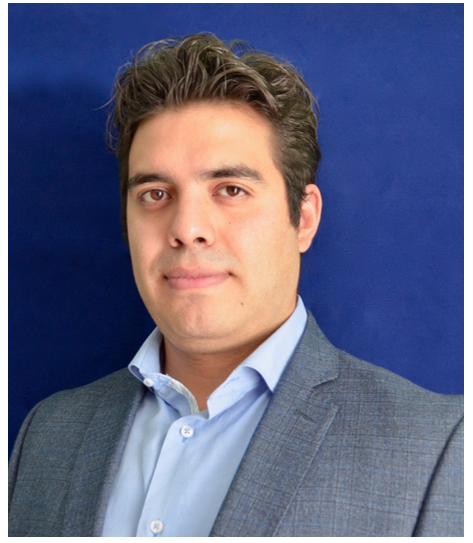
\includegraphics[width=6.57in]{img/00-presentacion/arturo} \end{center}

\textbf{ACT. KARINA LIZETTE GAMBOA}

\textbf{LinkedIn:} \href{https://www.linkedin.com/in/kalizzygam/}{KaLizzyGam}
\textbf{Email:} \href{mailto:lizzygamboa@ciencias.unam.mx}{\nolinkurl{lizzygamboa@ciencias.unam.mx}}

Actuaria egresada de la Facultad de Ciencias, por la UNAM y candidata a Maestra en
Ciencia de Datos por el ITAM.

Experiencia en áreas de analítica predictiva e inteligencia del negocio. Lead y Senior
Data Scientist en consultoría en diferentes sectores como tecnología, asegurador,
financiero y bancario. Es experta en entendimiento de negocio para la correcta
implementación de algoritmos de inteligencia y explotación de datos.
Actualmente se desarrolla como Arquitecta de Soluciones Analíticas en Merama,
startup mexicana clasificada como uno de los nuevos unicornios de Latinoamérica.
Senior Data Science en CLOSTER y como profesora del diplomado de Metodología
de la Investigación Social por la UNAM así como instructora de cursos de Ciencia de
Datos en AMAT.

Empresas anteriores: GNP, Activer Banco y Casa de Bolsa, PlayCity Casinos,
RakenDataGroup Consulting, entre otros.

\begin{center}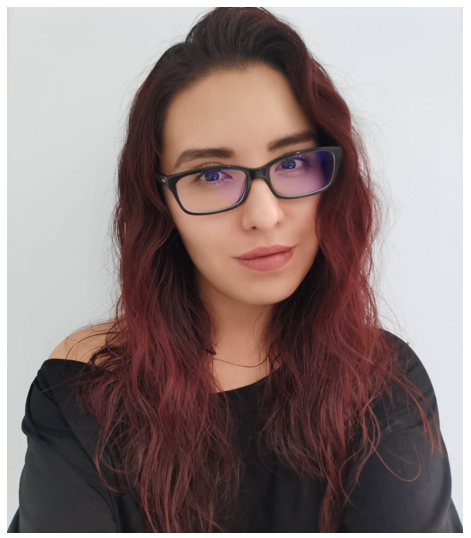
\includegraphics[width=250pt]{img/00-presentacion/lizzy} \end{center}

\hypertarget{temario}{%
\subsection*{Temario:}\label{temario}}
\addcontentsline{toc}{subsection}{Temario:}

\hypertarget{muxf3dulo-1-introducciuxf3n-a-r-22-hrs}{%
\subsubsection*{Módulo 1: Introducción a R (22 hrs)}\label{muxf3dulo-1-introducciuxf3n-a-r-22-hrs}}
\addcontentsline{toc}{subsubsection}{Módulo 1: Introducción a R (22 hrs)}

\textbf{Objetivo:} A través de este módulo se adquirirán los conocimientos necesarios para la operación del software estadístico y la manipulación ágil de datos. Al finalizar, el participante desarrollará análisis exploratorios y reportes automatizados.

\begin{itemize}
\item
  Estructuras de almacenamiento de datos

  \begin{itemize}
  \tightlist
  \item
    Almacenamiento
  \item
    Vectores
  \item
    Matrices
  \item
    Listas
  \item
    DataFrames
  \end{itemize}
\item
  Funciones y estructuras de control

  \begin{itemize}
  \tightlist
  \item
    Librerías y funciones
  \item
    Condicionamiento
  \item
    Ciclos
  \end{itemize}
\item
  Manipulación de estructuras de datos

  \begin{itemize}
  \tightlist
  \item
    Importación de tablas
  \item
    Consultas y transformación de estructuras
  \item
    Iteraciones
  \item
    Manipulación de texto y datos temporales
  \end{itemize}
\item
  Análisis exploratorio y visualización de datos

  \begin{itemize}
  \tightlist
  \item
    Guía de visualización
  \item
    Análisis Exploratorio de Datos (EDA)
  \item
    Análisis Gráfico Exploratorio de Datos (GEDA)
  \item
    Reportes con markdown
  \end{itemize}
\item
  Consultoría y aplicaciones con datos institucionales
\end{itemize}

\hypertarget{muxf3dulo-2-introducciuxf3n-a-ciencia-de-datos-18-hrs}{%
\subsubsection*{Módulo 2: Introducción a Ciencia de Datos (18 hrs)}\label{muxf3dulo-2-introducciuxf3n-a-ciencia-de-datos-18-hrs}}
\addcontentsline{toc}{subsubsection}{Módulo 2: Introducción a Ciencia de Datos (18 hrs)}

\textbf{Objetivo:} Este módulo presenta los conceptos teóricos clave para conocer los términos, objetivo y alcances de proyectos con enfoque en ciencia de datos. Se presenta el flujo de trabajo y organización que deberá seguir un equipo para obtener el mayor beneficio posible. Adicionalmente, se propone presentar el software git y github para implementar correctamente el trabajo en equipo que garantice la reproducibilidad y seguridad del desarrollo realizado.

\begin{itemize}
\item
  Introducción a ciencia de datos

  \begin{itemize}
  \tightlist
  \item
    ¿Qué es la ciencia de datos?
  \item
    Objetivo de ciencia de datos
  \item
    Requisitos y aplicaciones
  \item
    Tipos de algoritmos
  \item
    Ciclo de vida de un proyecto
  \item
    Taller de scoping
  \item
    Perfiles de un equipo de ciencia de datos
  \end{itemize}
\item
  Concepto de Ciencia de Datos

  \begin{itemize}
  \tightlist
  \item
    Machine learning
  \item
    Análisis supervisado
  \item
    Análisis no supervisado
  \item
    Sesgo y varianza
  \item
    Pre-procesamiento e ingeniería de datos
  \item
    Partición de datos
  \end{itemize}
\item
  Colaboración y reproducibilidad

  \begin{itemize}
  \tightlist
  \item
    Git \& Github
  \item
    Ambiente de desarrollo
  \end{itemize}
\item
  Consultoría y aplicaciones con datos institucionales
\end{itemize}

\hypertarget{muxf3dulo-3-machine-learning-supervisado-38-hrs}{%
\subsubsection*{Módulo 3: Machine Learning: Supervisado (38 hrs)}\label{muxf3dulo-3-machine-learning-supervisado-38-hrs}}
\addcontentsline{toc}{subsubsection}{Módulo 3: Machine Learning: Supervisado (38 hrs)}

\textbf{Objetivo:} Este módulo está diseñado para adquirir los conocimientos técnicos para conocer e implementar los distintos modelos de aprendizaje supervisado que son aplicados en ciencia de datos a la industria de los seguros y fianzas.

\begin{itemize}
\item
  Modelos de aprendizaje Supervisado

  \begin{itemize}
  \tightlist
  \item
    Regresión Lineal
  \item
    Regresión logística
  \item
    Regularización Ridge \& Lasso
  \item
    Elasticnet
  \item
    KNN
  \item
    Árbol de decisión
  \item
    Bagging
  \item
    Random Forest
  \item
    Boosting
  \item
    Stacking
  \end{itemize}
\item
  Toma de decisiones enfocadas a negocio

  \begin{itemize}
  \tightlist
  \item
    Comparación de modelos
  \item
    Balance entre sesgo y cobertura
  \item
    Cuantificación de sesgo e inequidad
  \item
    Cuantificación de ganancia comercial
  \item
    Diseño experimental
  \end{itemize}
\item
  Consultoría y aplicaciones con datos institucionales
\end{itemize}

\hypertarget{muxf3dulo-4-machine-learning-no-supervisado}{%
\subsubsection*{Módulo 4: Machine Learning: No Supervisado}\label{muxf3dulo-4-machine-learning-no-supervisado}}
\addcontentsline{toc}{subsubsection}{Módulo 4: Machine Learning: No Supervisado}

\textbf{Objetivo:} Este módulo permite al participante conocer técnicas de clustering para clasificar clientes de acuerdo con la utilidad y riesgo para la empresa. Adicionalmente, se presentan aplicaciones de clustering enfocadas a la estratificación de acuerdo con el riesgo geográfico.

\begin{itemize}
\item
  Técnicas de reducción de dimensión

  \begin{itemize}
  \tightlist
  \item
    Análisis de componentes principales
  \item
    Creación de índices
  \end{itemize}
\item
  Clustering

  \begin{itemize}
  \tightlist
  \item
    Liga simple, compleja y promedio
  \item
    Dendogramas \& heatmaps
  \item
    Kmeans \&
  \item
    Kmedoids
  \item
    DBSCAN
  \end{itemize}
\item
  Consultoría y aplicaciones con datos institucionales
\end{itemize}

\hypertarget{requisitos}{%
\subsection*{Requisitos:}\label{requisitos}}
\addcontentsline{toc}{subsection}{Requisitos:}

\begin{quote}
Computadora con al menos 4Gb Ram.
\end{quote}

\begin{quote}
Instalación de R con versión \textgreater= 4.1.0
\end{quote}

\begin{quote}
Instalación de Rstudio con versión \textgreater= 1.4.17
\end{quote}

\begin{quote}
Conocimientos generales de probabilidad, estadística y álgebra lineal
\end{quote}

\hypertarget{duraciuxf3n-y-evaluaciuxf3n-del-curso}{%
\section*{Duración y evaluación del curso}\label{duraciuxf3n-y-evaluaciuxf3n-del-curso}}
\addcontentsline{toc}{section}{Duración y evaluación del curso}

\begin{itemize}
\item
  El programa tiene una duración de 90 hrs.
\item
  Las clases serán impartidas los días lunes a viernes, de 7:00 am a 9:00 pm
\item
  Serán asignados ejercicios que el participante deberá resolver entre una semana y otra.
\item
  Al final del curso se solicitará un proyecto final, el cual \textbf{deberá ser entregado para ser acreedor a la constancia de participación}.
\end{itemize}

\hypertarget{recursos-y-dinuxe1mica-de-clase}{%
\section*{Recursos y dinámica de clase}\label{recursos-y-dinuxe1mica-de-clase}}
\addcontentsline{toc}{section}{Recursos y dinámica de clase}

En esta clase estaremos usando:

\begin{itemize}
\item
  R \href{https://cran.r-project.org/}{(descargar)}
\item
  RStudio \href{https://www.rstudio.com/products/rstudio/download/}{(descargar)}
\item
  Zoom \href{}{Clases}

  \begin{itemize}
  \tightlist
  \item
    \textbf{Pulgar arriba:} Voy bien, estoy entendiendo!
  \item
    \textbf{Pulgar abajo:} Eso no quedó muy claro
  \item
    \textbf{Mano arriba:} Quiero participar/preguntar ó Ya estoy listo para iniciar
  \end{itemize}
\item
  \href{}{Google Drive}
\item
  \href{https://acturio.github.io/amt22_aserta_intro2dsml/}{Notas de clase}
\item
  Finalmente, se dejarán ejercicios que serán clave para el éxito del aprendizaje de los capítulos, por lo que se trabajará en equipo para lograr adquirir el mayor aprendizaje.
\end{itemize}

  \bibliography{book.bib,packages.bib}

\end{document}
